\section{Implementation and development methodologies}
In this chapter, the inClass application is analyzed from the implementation point of view. As a quick remind, some general facts about the Rails framework will be mentioned, in order to understand better the listings presented bellow. Remember that  Rails follows the MVC  architectural pattern, which enforces a separation between “domain logic” (also called “business logic”) from the input and presentation logic, associated with a graphical user interface (GUI). In the case of web applications, the “domain logic” typically consists of data models for things like users, articles, and products, and the GUI is just a web page in a web browser.

When interacting with a Rails application, a browser sends a request, which is received by a web server and passed on to a Rails controller, which is in charge of what to do next. In some cases, the controller will immediately render a view, which is a template that gets converted to HTML and sent back to the browser. More commonly for dynamic sites, the controller interacts with a model, which is a Ruby object that represents an element of the site (such as a user) and is in charge of communicating with the database. After invoking the model, the controller then renders the view and returns the complete web page to the browser as HTML. This is the complete interaction process between Rails components. Now, it is the moment to get started with some details about how the functionality of inClass application was implemented. 

\subsection{Project configuration}
Assuming that the Ruby on Rails environment was already installed on the local machine, creating a new project is done by typing the command from \autoref{newproj} in the Terminal:

\begin{lstlisting}[style=nonumbers, caption={Create new Rails project},label={newproj}]
$ rails new student
\end{lstlisting}
\bigskip

This command creates a Rails application, called Student in a \texttt{student} directory and install the gem dependencies in \texttt{Gemfile}. The \texttt{student} directory has a number of auto-generated files and folders that make up the structure of a Rails application. Most of the work happened in the \texttt{app} folder. \autoref{table:new-project} presents a basic overview of each of the files and folders that Rails creates by default and their functions.

At this moment, a functional Rails application, called \texttt{Student} already exists on the local computer. To access it, it is necessary to start a web server on the development machine. This can be done by running the following command in the Terminal pointing to the \texttt{student} directory:

\begin{lstlisting}[style=nonumbers, caption={Navigate to localhost},label={localhost}]
$ bin/rails server
\end{lstlisting}

\begin{table}[H]
\centering
\caption{Auto-generated files in a Rails project}
\resizebox{\textwidth}{!}{\begin{tabular}{| c | l |}
\hline
\textbf{File/Folder} & \textbf{Purpose}\\
\hline
app/& Contains controllers, models, views, helpers, mailers and assets for the application.\\
\hline
bin/ & Contains the rails script that starts the app.\\
\hline
config/ & Configurations for the application's routes, database, etc.\\
\hline
config.ru & Rack configuration for Rack based servers used to start the application.\\
\hline
db/ & Contains the current database schema, as well as the database migrations.\\
\hline
Gemfile & Allows to specify what gem dependencies are needed for the Rails application.\\
\hline
lib/ & Extended modules for the application.\\
\hline
log/ & Application log files.\\
\hline
public/ & The only folder seen by the world as-is. Contains static files and compiled assets.\\
\hline
Rakefile & This file locates and loads tasks that can be run from the command line.\\
\hline
test/ & Unit tests, fixtures, and other test tools.\\
\hline
tmp/ & Temporary files (like cache, pid, and session files).\\
\hline
vendor/ & A place for all third-party code (vendored gems).\\
\hline
\end{tabular}}
\label{table:new-project}
\end{table}

To see the application in action, it is needed to navigate to \texttt{http://localhost:3000} via a web browser. Given the fact that the project is still empty, the Rails default information page is displayed. The \autoref{fig:rails-welcome} illustrates how the page actually looks like:

\begin{figure}[H]
\centering
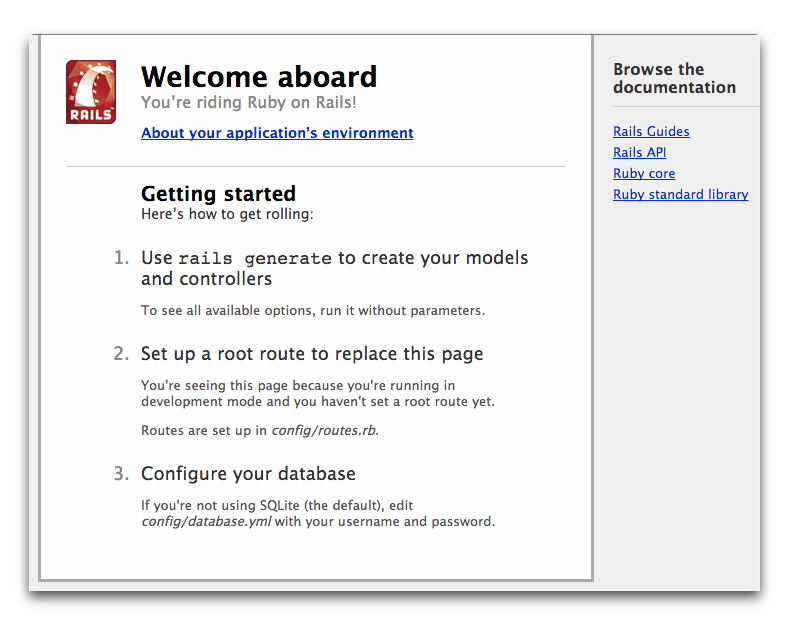
\includegraphics[width=12cm]{Chapter3/rails_welcome.png}
\caption{Rails Welcome page}
\label{fig:rails-welcome}
\end{figure}

The "Welcome aboard" page is the basic test for a new Rails application: it makes sure that the development software is configured correctly enough to serve a page. Hitting \texttt{Ctrl+C} in the terminal window where the server runs will stop the web server.

\subsection{Back-end implementation of the application}
To get Rails store, display and change data, it is needed to create minimum a model, a controller and a view. As example will serve the development of the system's \texttt{University} component. Given the fact that this entity is supposed to allow storing instances, a \texttt{University} model should be created. To do this, the command in \autoref{model-gen} has to be executed in Terminal:

\begin{lstlisting}[style=nonumbers, caption={Generate model University},label={model-gen}]
bin/rails generate model University
\end{lstlisting}
\bigskip

According to Active Record conventions, models in Rails use a singular name, and their corresponding database tables use a plural name. After running \texttt{bin/rails generate model}, a database migration file will be created inside the \texttt{db/migrate} directory. Migrations are Ruby classes that are designed to make it simple to create and modify database tables. Rails uses rake commands to run migrations, and it's possible to undo a migration after it's been applied to a database. Migration filenames include a timestamp to ensure that they're processed in the order that they were created.

The \autoref{university-migration} offers a look inside the recently generated migration. It can be observed that a series of attributes were added to the \texttt{universities} table in the database, which is mapped to the \texttt{University} model. Active Record is smart enough to automatically map column names to model attributes, which means there is no need to declare attributes inside Rails models, as that will be done automatically by Active Record.

\begin{lstlisting}[caption={Migration for Creating University},label={university-migration}]
class CreateUniversities < ActiveRecord::Migration
  def change
    create_table :universities do |t|
      t.timestamps null: false
      t.string :title
    end
  end
end
\end{lstlisting}
\bigskip
 
The above migration creates a method named \texttt{change} which will be called when running this migration. The action defined in this method is also reversible, which means Rails knows how to reverse the change made by this migration, in case of reversing later. Running this migration will create an \texttt{universities} table with one string column. It also creates a timestamp field to allow Rails track university creation and update times.At this point, a rake command has to be used to run the migration and create the \texttt{universities} table, together with its attributes:

\begin{lstlisting}[style=nonumbers, caption={Add University table in the Database},label={migrate-university}]
$ bin/rake db:migrate
\end{lstlisting}
\bigskip

The procedure of generating the database is equivalent for the rest of the components in the application. The same steps were executed for creating faculties, specialties, timetables, groups, courses, students, teachers and admins. Completing this phase means the successful modeling of the data layer, resulting in a reliable structure for storing records.

The project contains several special models, which have Devise authentication attached. As mentioned above, Devise is a gem for Rails, bringing a high-level solution that takes care of many different aspects for implementation. It presents controllers, views, mailers, and routes. While it's simple to issue a couple of commands and have Devise up and running, it is highly customizable. Devise has very thorough documentation and a large community that produces a boatload of useful extensions. The gem comes with handful modules, allowing to choose only the required ones. As seen in the application's schema and model (Listings \ref{teacher-schema} and \ref{teacher-model}), after Devise was added to the Teacher component,  several modules were also generated to support password recovery, e-mail confirmation, account lock out, and many others. Bellow, an illustration of the application's schema, regarding the Teacher entity, is presented:

 \begin{lstlisting}[caption={Teacher Schema using Devise},label={teacher-schema}]
ActiveRecord::Schema.define(version: 20160514113821) do

  create_table "teachers", force: :cascade do |t|
    t.datetime "created_at",                          null: false
    t.datetime "updated_at",                          null: false
    t.string   "name"
    t.string   "teacher_faculty"
    t.string   "teacher_department"
    t.integer  "university_id"
    t.string   "email",                  default: "", null: false
    t.string   "encrypted_password",     default: "", null: false
    t.string   "reset_password_token"
    t.datetime "reset_password_sent_at"
    t.datetime "remember_created_at"
    t.integer  "sign_in_count",          default: 0,  null: false
    t.datetime "current_sign_in_at"
    t.datetime "last_sign_in_at"
    t.string   "current_sign_in_ip"
    t.string   "last_sign_in_ip"
  end

  add_index "teachers", ["email"], name: "index_teachers_on_email", unique: true
  add_index "teachers", ["reset_password_token"], name: "index_teachers_on_reset_password_token", unique: true

end
\end{lstlisting}
\bigskip

Also, several changes were generated in the Teacher model file, regarding the possible options that can be implemented, using Devise. The original code implied only database relations between tables, assuming that a Teacher can belong only to one University and can have only one timetable assigned. After Devise integration, the model became suitable for authentication, as seen bellow:

\begin{lstlisting}[caption={Teacher Model using Devise},label={teacher-model}]
class Teacher < ActiveRecord::Base
  	# Include default devise modules. Others available are:
  	# :confirmable, :lockable, :timeoutable and :omniauthable
  	devise :database_authenticatable, :recoverable, :rememberable, :trackable, :validatable
	belongs_to :university
	has_one :timetable
end

\end{lstlisting}
\bigskip

In the discussed project, the Admin model, the Teacher model and the Student model have the authentication resource provided by Devise. Once the database is set up, controllers need to be created. As example, in the \autoref{university-controller-new} is presented the command that is used to generate a new controller:

\begin{lstlisting}[style=nonumbers, caption={Generate controller University},label={university-controller-new}]
bin/rails generate controller Universities
\end{lstlisting}
\bigskip

The fresh University Controller handles taking the input data from the URL (or the request body in the case of POST and PUT) and then interacts with the Model, as well as setting up data for the view portion. By default, Rails emphasizes a “RESTful” approach; that is to say, it uses the given HTTP verb (for example, GET, POST, PUT, DELETE) and well-organized urls to represent resources, leading to a general structure where code goes for operations on an object. It provides tools to handle basic CRUD (Create, Read, Update, Delete) actions on your data. In Rails terminology, the actions are typically:
\begin{itemize}
\item index - An action that returns a listing of all resources; for example GET /universities will hit the index action on the Universities Controller, listing the known universities.
\item show - An action that performs a read operation for a single resource; for example GET /universities/1 will hit the show on the Universities Controller, showing the details of the University with id 1.
\item new - The action to show a new object form, in our case, the new University form; for example GET /universities/new will hit the new action on the Universities Controller and show the new University form.
\item create - A post action to take the form data from the new action and to attempt to create a record; for example POST /universities will hit the create action on the Universities Controller, typically with some associated form data.
\item edit - Will show the form to edit a specific resource; for example GET /universities/1/edit will hit the edit action on the Universities Controller and show a form to edit the URL with id 1.
\item update - Will attempt to update the given resource; for example PUT /universities/1 will hit the update action on the URLs Controller and attempt to update the University with id 1.
\item destroy - Will attempt to destroy a given resource; for example DELETE /universities/1 will hit the destroy action on the Universities Controller and attempt to destroy the University with id 1.
\end{itemize}

So, a resourceful route provides a mapping between HTTP verbs and URLs to controller actions. By the convention mentioned above, each action also maps to particular CRUD operations in a database. A single entry in the routing file such as \texttt{resources :universities} creates seven different routes in the application, all mapping to the University Controller:

\begin{table}[H]
\centering
\caption{Routes mapping the actions from University Controller}
\resizebox{\textwidth}{!}{\begin{tabular}{| c | l | l | l |}
\hline
\textbf{HTTP Verb} & \textbf{Path} & \textbf{Controller\texttt{\#}Action} & \textbf{Used for}\\
\hline
GET & /universities & \texttt{universities\#index} & display a list of all universities\\
\hline
GET & /universities/new & \texttt{universities\#new} & return HTML form for creating an university\\
\hline
POST & /universities & \texttt{universities\#create} & create a new university\\
\hline
GET & /universities/:id & \texttt{universities\#show} & display a specific university\\
\hline
GET & /universities/:id/edit & \texttt{universities\#edit} & return HTML form for editing an university\\
\hline
PATCH/PUT & /universities/:id & \texttt{universities\#update} & update a specific university\\
\hline
DELETE & /universities/:id & \texttt{universities\#destroy} & delete a specific university\\
\hline
\end{tabular}}
\label{table:routes-university}
\end{table}

For better understanding, in \autoref{routes-university} are presented all the resources and their routes that were created for the project. Can be observed the multiple namespaces used for each category of user. The namespaces help divide the application's functionality, depending on the resources allowed for a given user:

\begin{lstlisting}[caption={Application's resources routes},label={routes-university}]
Rails.application.routes.draw do

  devise_for :scholars, :controllers => {:sessions => 'scholar/sessions'}
  devise_for :teachers, :controllers => {:sessions => 'teacher/sessions'}
  devise_for :admins

  namespace :admin do
    get '/' => 'home#index'
    resources :teachers, only: [:index, :show]
    resources :faculties, only: [:index, :show]
    resources :specialties, only: [:index, :show]
    resources :groups, only: [:index, :show]
    resources :universities do
      resources :teachers, except: [:index, :show]
      resources :faculties, except: [:index, :show] do
        resources :specialties, except: [:index, :show] do
          resources :groups, except: [:index, :show] do
            resources :timetables do
              resources :courses
            end
          end
        end
      end
    end
  end

  namespace :teacher do
    get '/' => 'home#index'
    resources :timetables
  end

  namespace :scholar do
    get '/' => 'home#index'
    resources :timetables
    get 'profile' => 'profiles#show', as: :profile
    get 'profile/edit' => 'profiles#edit', as: :edit
    match 'profile/update' => 'profiles#update', as: :update, via: [:put, :patch]
  end

  root 'home#index'
\end{lstlisting}
\bigskip

Given the fact that the current University Controller needs all the actions implemented in order to be able to create, edit, show and destroy an instance, the content of the corresponding file looks like this:

\begin{lstlisting}[caption={Content of University Controller},label={university-controller}]
class Admin::UniversitiesController < AdminsController
  def index
    @universities = University.all
  end

  def show
    @university = University.find(params[:id])
  end

  def create
    @university = University.new(university_params)
    if @university.save
      redirect_to admin_universities_path(@university)
    end
  end

  def new
    @university = University.new
    respond_to :html, :js
  end

  def edit
    @university = University.find(params[:id])
    respond_to :html, :js
  end

  def update
    @university = University.find(params[:id])
    if @university.update university_params
      redirect_to :action => 'index', :id => @university
    else
      render :edit
    end
  end

  def destroy
    @university = University.delete(params[:id])
    redirect_to :action => :index
  end

  private
  def university_params
    params.require(:university).permit(:title)
  end
end
\end{lstlisting}
\bigskip

The rest of the controllers (Faculty Controller, Specialty Controller, Group Controller, Timetable Controller, Course Controller, Student Controller, Teacher Controller, Admin Controller) follow the same principle of creation and action implementation, depending on the needs it has to accomplish. Besides the controllers that need to be created, there is still one that wasn't mentioned until now. This is the Application Controller, which is generated at the creation moment of the Student application. Given the fact that the system operates with different namespaces, for better structuring of the project, some configuration where needed to be specified in this controller. Detailed information is presented in \autoref{application-controller}:

\begin{lstlisting}[caption={Content of Application Controller},label={application-controller}]
class ApplicationController < ActionController::Base
  before_action :configure_permitted_parameters, if: :devise_controller?
  protect_from_forgery with: :exception

  protected
  def after_sign_in_path_for (resource)
  	if resource.class == Admin 
  		stored_location_for(resource) || admin_path
  	elsif resource.class == Teacher
  		stored_location_for(resource) || teacher_path	
    elsif resource.class == Scholar
      stored_location_for(resource) || scholar_path 
    end
  end

  def after_sign_up_path_for (resource)
    if resource.class == Admin 
      stored_location_for(resource) || admin_path
    elsif resource.class == Teacher
      stored_location_for(resource) || teacher_path
    elsif resource.class == Scholar
      stored_location_for(resource) || scholar_path 
    end
  end

  def configure_permitted_parameters
    devise_parameter_sanitizer.for(:sign_up){|u| u.permit(:email, :password, :password_confirmation, :group_id)}
  end
\end{lstlisting}
\bigskip

These three methods are responsible for proper resource rendering, depending on the type of user. The methods are implemented for  log in and log out activity. The third method is responsible for student's registration, specifying the permitted parameters. The first two params are Devise - related, while the third one was manually included for ensuring the connection between student and its membership group.

\subsection{Front-end implementation of the application}
A Rails View is an ERb (Embedded Ruby) program that shares data with controllers through mutually accessible variables.If the app/views directory of the Student application is accessed, one subdirectory for each of the created controllers can be seen. Each of these subdirectories is created automatically when the same-named controller is created with the generate script. Each method defined in the controller needs to have a corresponding \texttt{erb} file, with the same name as the method, to display the data that the method is collecting (except for the delete method, where no view is needed). In the current project, another gem was used in order to transform all \texttt{erb} files in \texttt{haml} files, which simplifies things for the coding process. So, for the University Controller, 4 views were generated. The first one to be analyzed is the \texttt{new} view. It contains the form for creating a new University instance, as shown in \autoref{university-new-form}. Actually, the views can not be considered as front-end components, but the fragments of code presented in this section are combined with front-end elements, as the system's development is currently finished. 

\begin{lstlisting}[caption={Form for creating a new University},label={university-new-form}]
= form_for [:admin, @university] do |f|
  = f.text_field :title, :class => "input-form-edit"
  = f.submit :class => "btn btn-default add-btn-default"
\end{lstlisting}
\bigskip

 Assuming that the University is defined as having only one attribute - title - in the database, the form contains only the text field, where the name can be typed in. The other element is the "Submit" button, for saving the new instance. It can be observed that these two elements are using two CSS classes for the front-end part. 
 
These classes are located in the \texttt{student/app/assets/stylesheet/layout/admin} directory, following the convention about structuring front-end files. \autoref{css-class} is displaying the content of the "input-form-edit" and  "btn btn-default add-btn-default" classes.
 
 \begin{lstlisting}[caption={CSS classes for the University instance},label={css-class}]
.input-form-edit{
	margin-bottom: 15px; 
	height: 40px;
	font-size: 16px;
	font-family: $font_lato;
}

.btn{
	&.btn-default{
		font-family: $font_lato;

	}
	&.add-btn-default{
		margin-top: 15px;
	}

	&.select-btn-default{
		margin-top: 15px;
	}
\end{lstlisting}
\bigskip

The \texttt{.btn} class consists of 3 children classes, which are applied to different types of buttons in the application. This technique permits code reuse by avoiding the creation of separate classes and keeps up with the DRY(Don't Repeat Yourself!) principle during the system implementation. For rendering the \texttt{new} form in the current page, JavaScript language was used:

\begin{lstlisting}[style=nonumbers, caption={Render form in current page using Javascript},label={university-new-form-javascript}]
var newUniversity = $('#new-university')
newUniversity.html('<%=j render partial: "new" %>')
\end{lstlisting}
\bigskip

The \texttt{\#new-university} variable is an \texttt{id} used in the University's show page where the form has to be rendered. Its position indicates the specific location in the page where the form has to be inserted. The \texttt{edit} view is similar with the \texttt{new} one, that's why it is skipped. 

The next view to be discussed is the \texttt{index} view. For the design part of this page Bootstrap classes were used. For similar pages, the same concept was followed. The file presented bellow displays the page containing all the available current universities. \autoref{university-show-view} comes with implementation details:

\begin{lstlisting}[caption={Index view of the University instance},label={university-show-view}]
.container
  .col-md-9.col-md-offset-1
    .row
      %h1.text-center.heading-font
        All universities
      = link_to(new_admin_university_path, :method =>:get, :remote => true, :class => "icon-left add-button") do
        %span
          Add university
      #new-university
      %hr
      - @universities.order(:title).each do |u|
        %ul.action-block
          .col-md-6
            %li
              %b
                = link_to u.title, {:controller => :universities, :action => :show, :id => u.id, :method => :get}
          .col-md-3
            %li
              = link_to({:controller => :universities, :action => :edit, :id => u.id}, :class =>"icon-left edit-button", :method => :get, :remote => true) do
                %span
                  Edit university
            .edit-university{:id => "edit-university-#{u.id}"}
          .col-md-3
            %li
              = link_to({:controller => :universities, :action => :destroy, :id => u.id}, :class =>"icon-left delete-button", :method => :delete) do
                %span
                  Delete university
        %hr

\end{lstlisting}
\bigskip

From the code listed above, it is seen that some additional CSS classes were used for buttons style, which implies icon positioning in the left-side of the actual button. The "icon-left", presented in \autoref{icon-left-css} class also has child classes, that have specific implementations for every type of button in the application. 

\begin{lstlisting}[caption={CSS classes used for buttons design},label={icon-left-css}]
.icon-left{

	&:before{
			content: "";
			width: 18px;
			height: 18px;
			float: left;
			display: inline-block;
	}

	&.delete-button{
		&:before{
			background-image: asset-url('delete.png');
		}
	}

	&.edit-button{
		&:before{
			background-image: asset-url('edit.png');
		}
	}

	&.add-button{
		&:before{
			background-image: asset-url('add.png');
		}
	}
}
\end{lstlisting}
\bigskip

Speaking about the front-end applied strategies, the \texttt{show} page of the University follows the same principle as the \texttt{index} page, that's why further details are not presented in the paper work. 

\subsection{User's experience handling the product}
Another checkpoint in the development of an application is the user experience, described as the way a person feels about using a certain product. Performing such a procedure usually highlights some important aspects of the human-computer interaction and product ownership. It also creates some first impressions judging by the visual style of the product. For best results, the interaction with it should be as simple as possible. To increase the quality of the application, it is recommended to continuously  work on requirements, based on information gathered from user's feedback. In order to meet this goal, a set of possible questions from the user's side were generated. These questions include all the basic functionality the users expect to face while interacting with the application. Giving simple answers to those questions, improve the general user's opinion about the product. Find the questions listed bellow:
\begin{itemize}
\item What are the prerequisites in order to be able to use the application?
\item Who are the users of the application?
\item What is the format for student registration?
\item What is the format for teacher registration?
\item When is the application ready for use?
\item Who populates the database with records?
\item Who is responsible for database maintenance?
\item How to create a specific entity into the system?
\item What is the structure of the system?
\item What is the format of the course creation?
\item What kind of information should be prepared in advance for database population?
\item What is the validity period of the database records?
\end{itemize}

Thinking from user's point of view, a good product means a friendly user interface for interaction. inClass was thought as an easy to comprehend application, that would guarantee an easy access to the main components. That's why, for the first version, it was chosen to display data in the most accessible structure, via tabular representation. 

\subsubsection{Using the application as administrator}
The system was designed to look like other familiar application, which would intuitively guide the users through its components. Some of the basic activities that the users can perform during a session with inClass are presented bellow as application screenshots. In \autoref{fig:admin-login} is shown the first steps made by the administrator in order to access the system:

\begin{figure}[H]
\centering
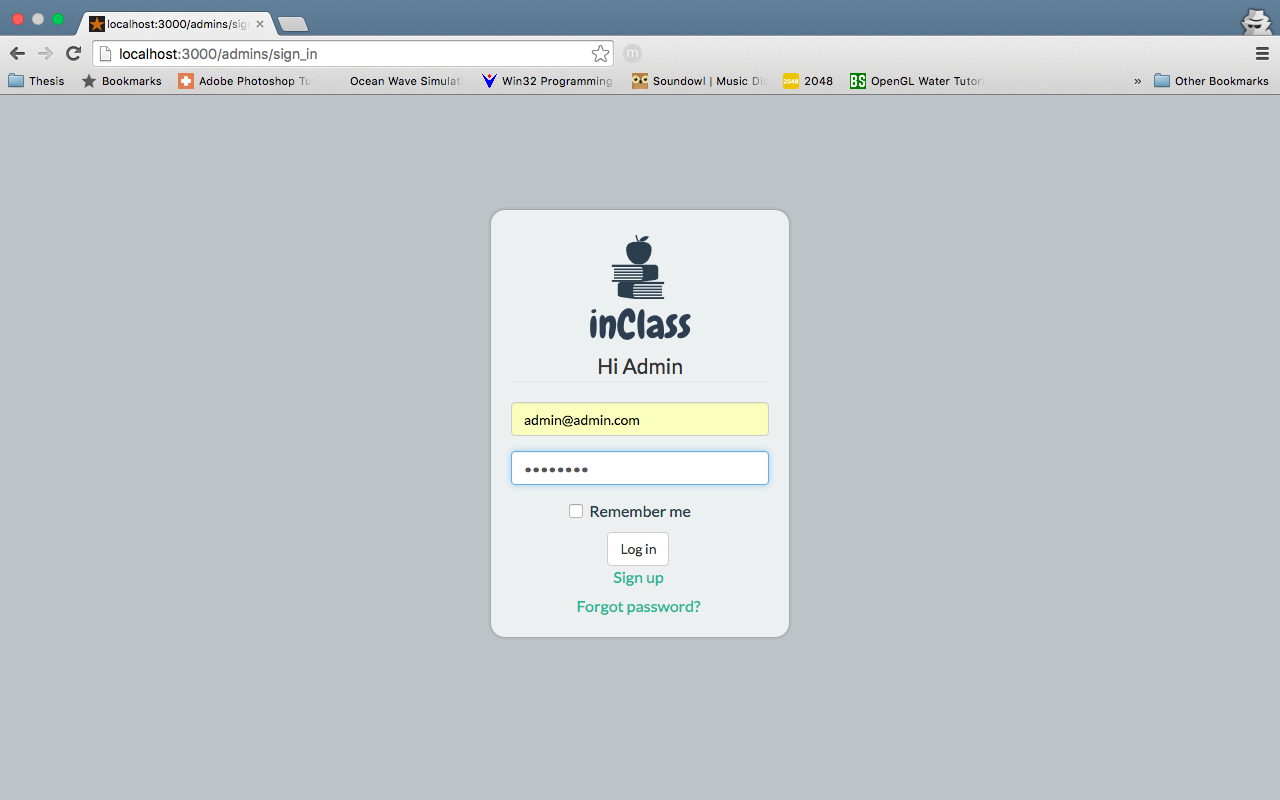
\includegraphics[width=14cm]{Chapter3/admin-login.png}
\caption{Admin log-in form}
\label{fig:admin-login}
\end{figure}

Given the fact that the application wasn't yet deployed, in order to reach it, the server has to be started from Terminal. After the necessary command was typed in, the administrator has to open a local browser and navigate to the address \texttt{http://localhost:3000}. Because the administrator side of the application is hidden from the standard users, the admin has to add to the url address a \texttt{/admin} missing piece of text for reaching the log in form.

After successful log-in, the admin can start creating the entities, which have a tree representation, where the main node is the university. The \autoref{fig:admin-university-add} illustrates how new universities are created.

\begin{figure}[H]
\centering
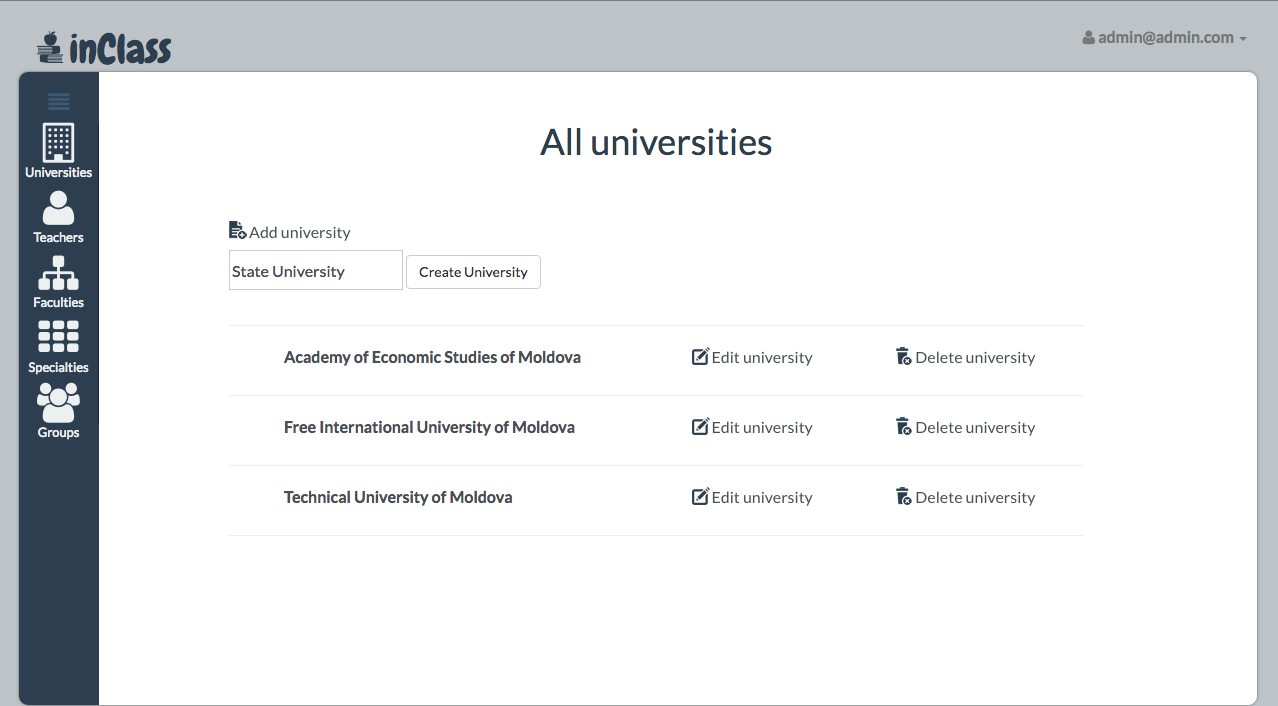
\includegraphics[width=14cm]{Chapter3/admin-university-add.png}
\caption{Adding new universities process}
\label{fig:admin-university-add}
\end{figure}

 Also, as mentioned above, the administrator is responsible for registering teachers into the system. In \autoref{fig:admin-teacher-add} is shown how a new teacher account is added:

\begin{figure}[H]
\centering
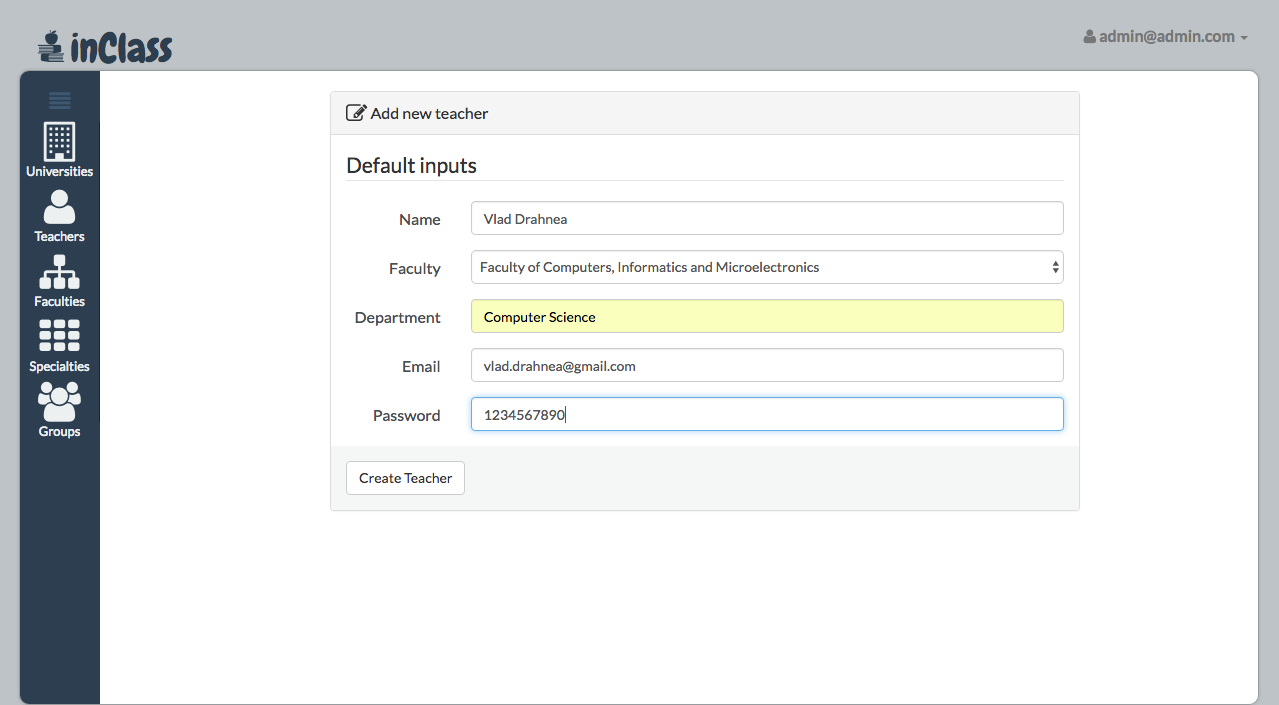
\includegraphics[width=14cm]{Chapter3/admin-teacher-add.png}
\caption{Teacher registration}
\label{fig:admin-teacher-add}
\end{figure}

The process of adding new faculties, specialties, groups and timetables is similar with the one of adding new universities, that's why additional screenshots were skipped. At this moment, the next process that is worth mentioning is the creation of courses, as parts of a timetable. This activity is represented in \autoref{fig:admin-course-add}:

\begin{figure}[H]
\centering
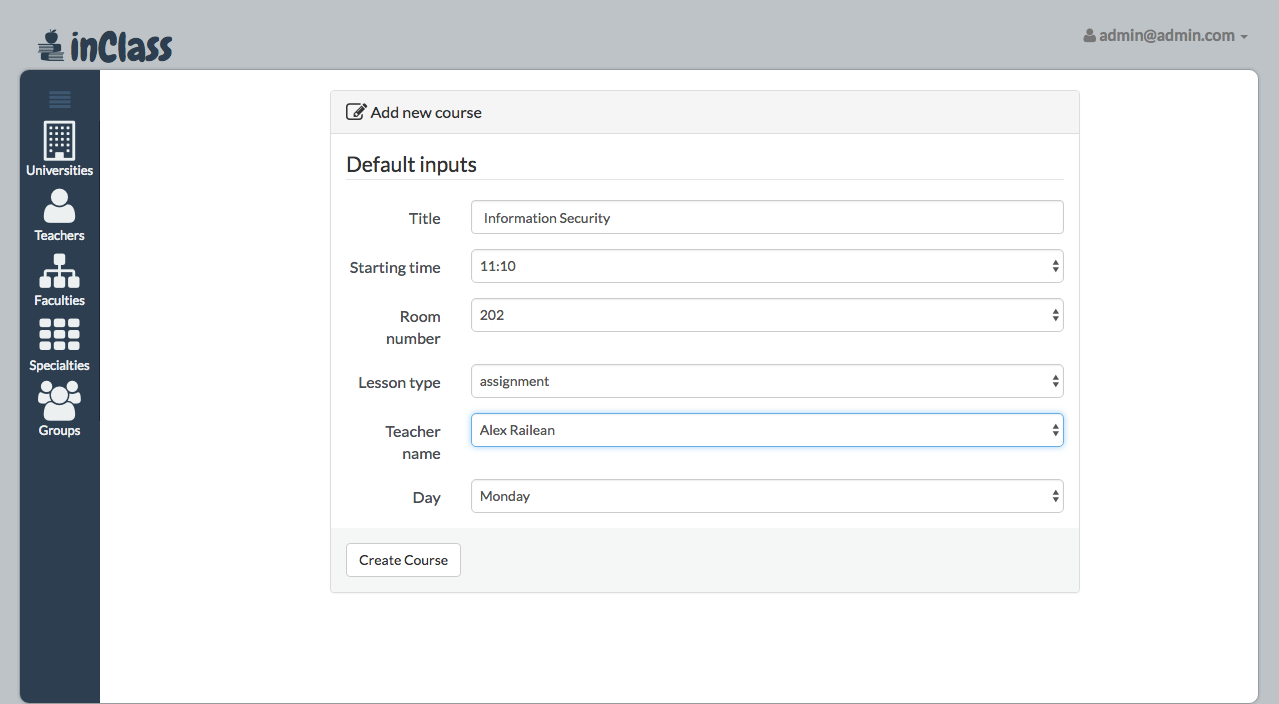
\includegraphics[width=14cm]{Chapter3/admin-course-add.png}
\caption{Form for adding a new course}
\label{fig:admin-course-add}
\end{figure}

For accessibility purposes, the menu in the left-side of the application contains links to ease the access to the in-depth layers, like groups, timetables and eventually - courses. So, to check his/her last activity, the administrator can avoid traversing the long path in order to reach the courses by clicking the appropriate link in the menu. The records are displayed in ascending order according to the last activities performed on each of them.
 
As a final step, adding all the necessary courses, results in a completely digitized timetable, available for any student subscribed as member of the group for which the timetable was created. The \autoref{fig:admin-timetable-show} illustrates how a timetable is displayed for the admin, and later - for students:

\begin{figure}[H]
\centering
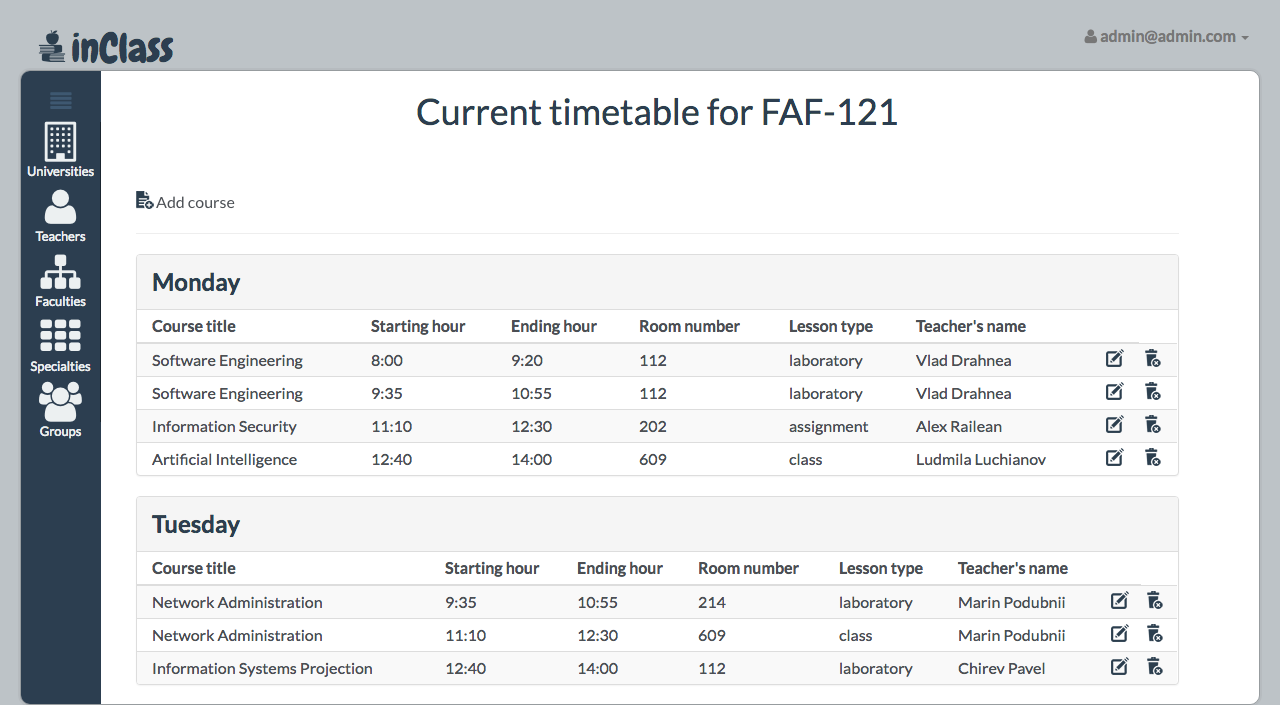
\includegraphics[width=14cm]{Chapter3/admin-timetable-show.png}
\caption{Final representation of a timetable for admin}
\label{fig:admin-timetable-show}
\end{figure}

This is the schematic representation of the admin side of the application. For the design part, it is reminded the fact that Hierapolis theme was integrated. There still remains to discuss the student-teacher side of the application, where the design was created from scratches and modeled using Bootstrap and CSS - written classes for the front-end part. 

\subsubsection{Using the application as teacher/student}
Assuming that the administrator has already created accounts for a specific group of teacher, let's log in the system with his/her credentials. In \autoref{fig:home} is presented the common home page, which stores the both possibilities of log in, for teachers and for students:

\begin{figure}[H]
\centering
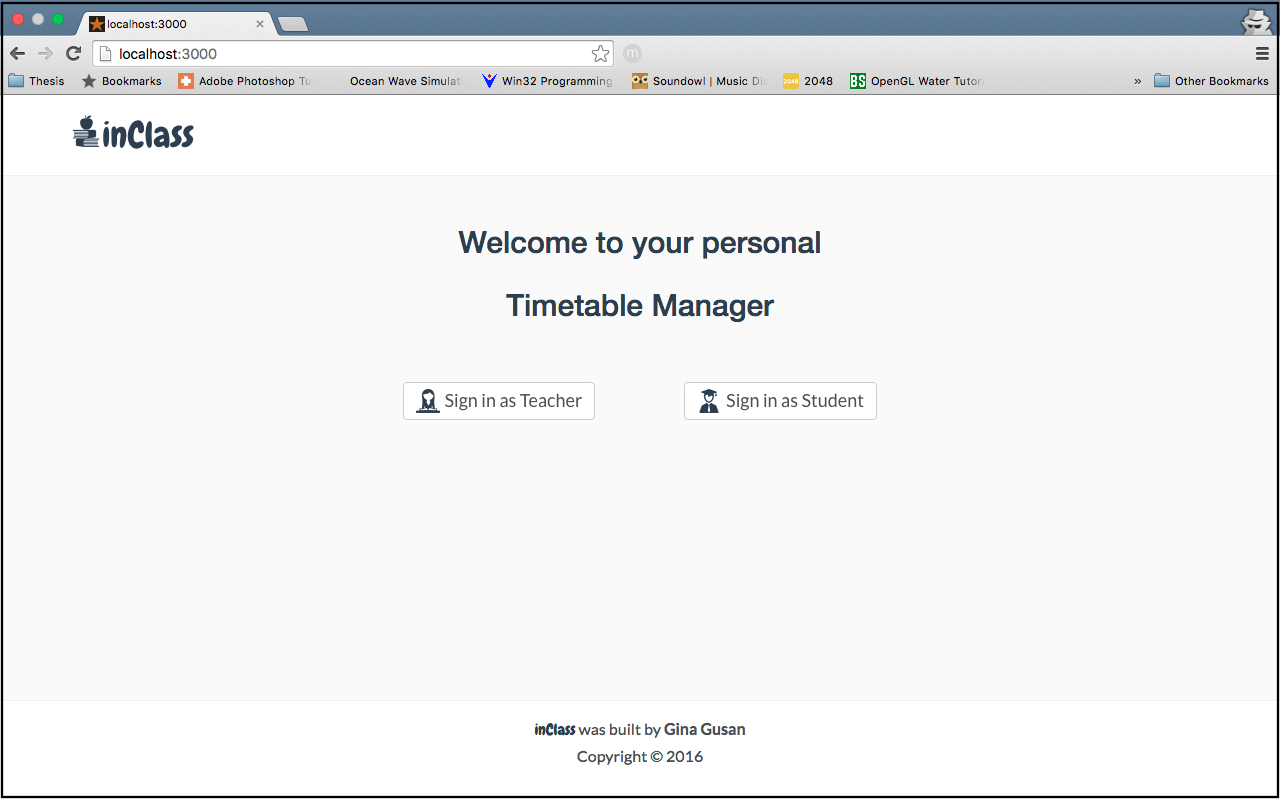
\includegraphics[width=14cm]{Chapter3/home.png}
\caption{Home page of the application}
\label{fig:home}
\end{figure}

After clicking the "Sign in as Teacher" button, the corresponding form will be rendered. The \autoref{fig:teacher-login} illustrates how the form actually looks like. It can be seen that, for having access in the system, every teacher has to receive a password that matches his email address. 

\begin{figure}[H]
\centering
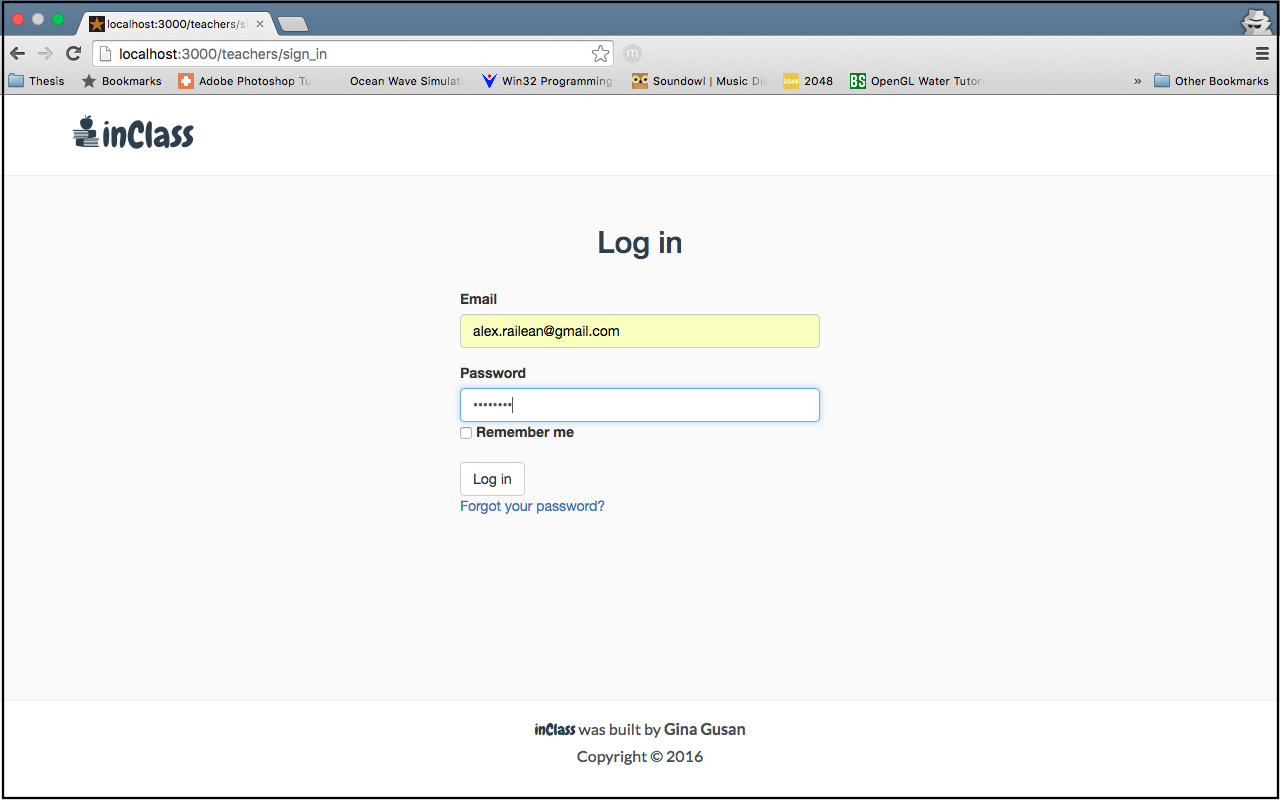
\includegraphics[width=14cm]{Chapter3/teacher-login.png}
\caption{Teacher's log in form}
\label{fig:teacher-login}
\end{figure} 

As a matter of fact, the forms for teacher and student are similar, with one exception, that the student has one additional button that gives the possibility to register into the system. Each student is responsible for personal registration, where he/she specifies for what group he wants his timetable to be generated. The \autoref{fig:student-signup} presents this distinctive situation:

\begin{figure}[H]
\centering
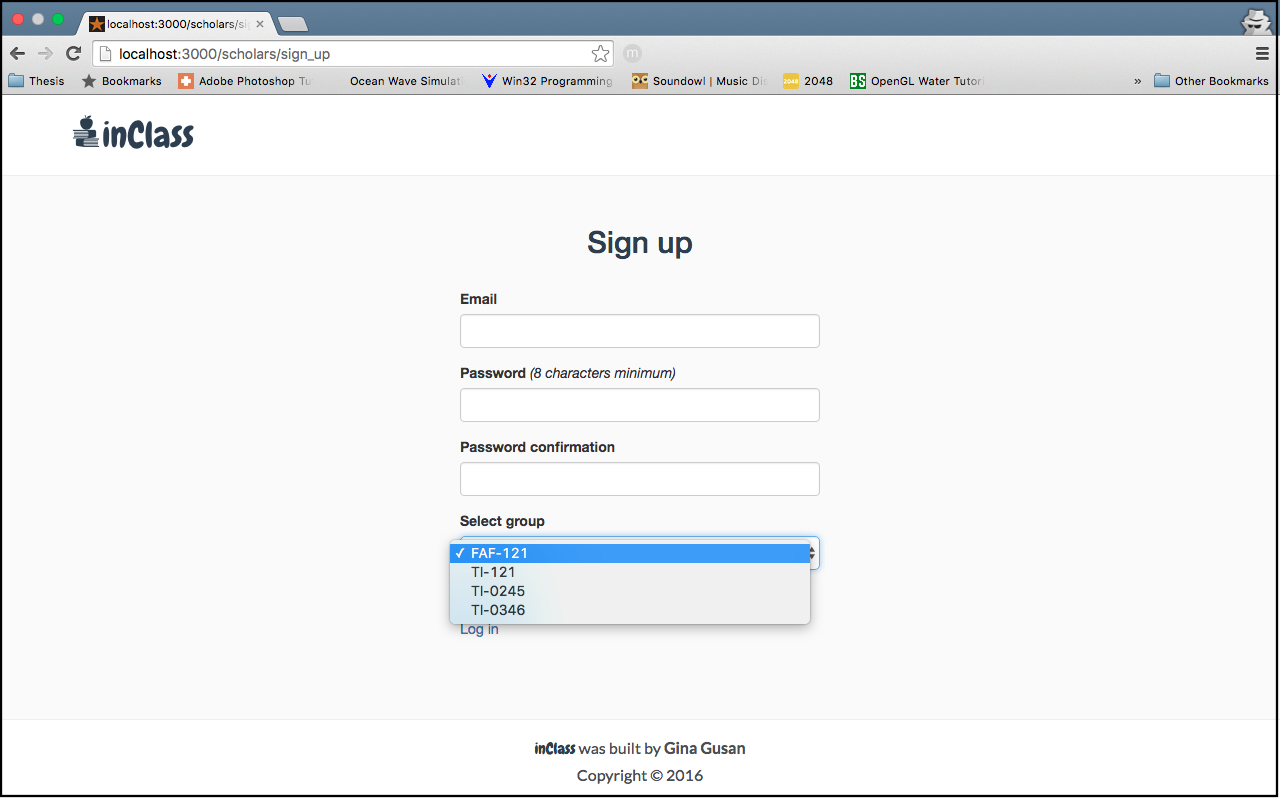
\includegraphics[width=14cm]{Chapter3/student-signup.png}
\caption{Student's sign up form}
\label{fig:student-signup}
\end{figure}

After logging in the system, the teacher is redirected to his home page, which displays his current timetable. The application compares the system's current day and selects only the courses that have this day specified at the time of creation. Bellow, is presented the result of this selection, for the current teacher:

\begin{figure}[H]
\centering
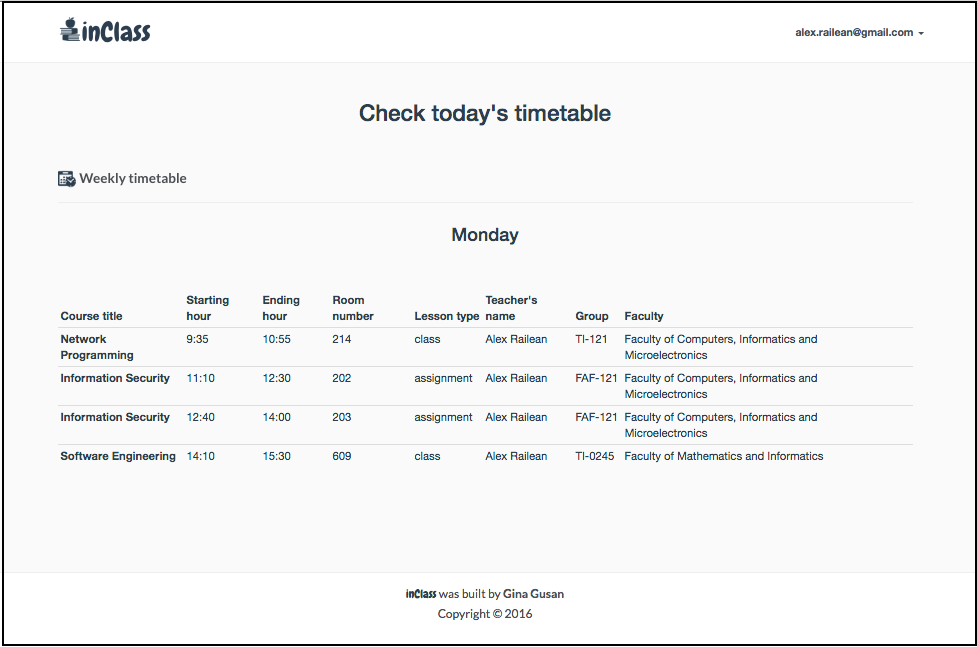
\includegraphics[width=14cm]{Chapter3/teacher-current-timetable.png}
\caption{Teacher's current timetable}
\label{fig:teacher-current-timetable}
\end{figure}

The process is equivalent for the student as user of the system, the only difference being that the "Faculty" and "Group" columns were omitted from the listing, from obvious reasons. 
In \autoref{fig:teacher-current-timetable} can be observed the button "Weekly Timetable" that, when it is clicked, redirect the teacher to the courses full schedule, where he/she can visualize the daily courses grouped by day and sorted in ascending order from the first working day until the last one. The \autoref{fig:teacher-weekly-timetable} presents that situation:

\begin{figure}[H]
\centering
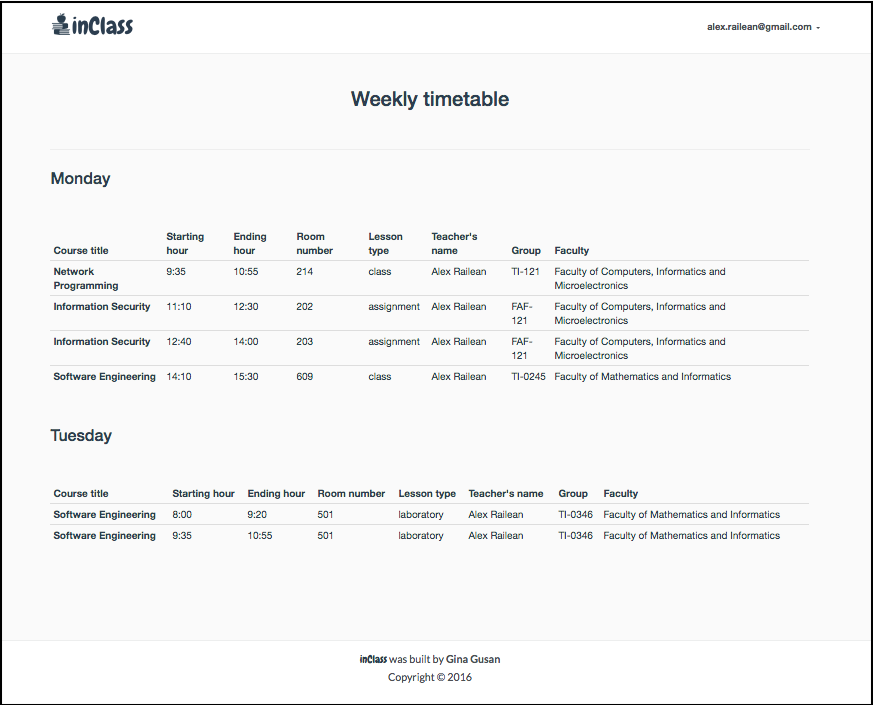
\includegraphics[width=14cm]{Chapter3/teacher-weekly-timetable.png}
\caption{Teacher's weekly timetable}
\label{fig:teacher-weekly-timetable}
\end{figure} 

At this point, the interaction between the system and each type of user is completed. Basically, all the functionality was covered and presented bellow. The next pending task to be implemented in the application's functionality is the sorting of timetable's courses by even and odd weeks. This particularity is encountered only at the Technical University of Moldova, that's why, in general lines the product is ready for release on the local market.

